\graphicspath{{lit_study/fig/}}

{
\tikzset{external/figure name/.add={lit_study/}{}}

\glsresetall % Restart gls entries and display full expansion of first entry again.

\chapter{Literature study} \label{chap:lit_study}

    \paragraph
    This chapter will present a study of the literature regarding the transportation of payloads with multirotors.
    Firstly, an overview of different payload configurations and control techniques for transporting payloads will be discussed.
    This study will specifically focus on control techniques that consider unknown, cable-suspended payloads.
    Furthermore, the different system identification methods for multirotor-payload systems will be discussed.
    This chapter will conclude with a summary of the considered literature and will compare it the to focus of this thesis.

\section{Payload transportation with multirotors}

    \paragraph
    The transportation of payloads with \glspl{UAV} has significantly grown in popularity over recent years.
    % Examples of specific applications of \gls{UAV} transportation include package deliveries \cite{}, pesticide application in agriculture \cite{}, and 
    Multirotor \glspl{UAV} are specifically useful for many transportation applications due to their agility, and their \gls{VTOL} capability.
    The types of payloads attached to multirotors can usually be categorised as either sensors (e.g.~cameras and meteorological sensors), or freight (e.g.~mail parcels or fire extinguishing material) \cite{Vergouw2016}.
    Furthermore, the payload attachment is mainly categorised as either a rigid connection, or a cable-suspended connection \cite{Vergouw2016}.
    In rare cases, a robotic actuator is attached to the multirotor to manipulate the payload \cite{Gonzalez-deSantos2020, Suthar2021}.
    The payload attachment and physical properties of the payload influence the multirotor flight dynamics and need to be considered for control system design.   
    % In many applications, some aspects of the payload configuration are unknown prior to flight and the control architecture needs to account for these unknowns.

    \begin{figure}
        \captionsetup[subfigure]{justification=centering}
        \centering  
        \begin{subfigure}[t]{0.32\textwidth}
            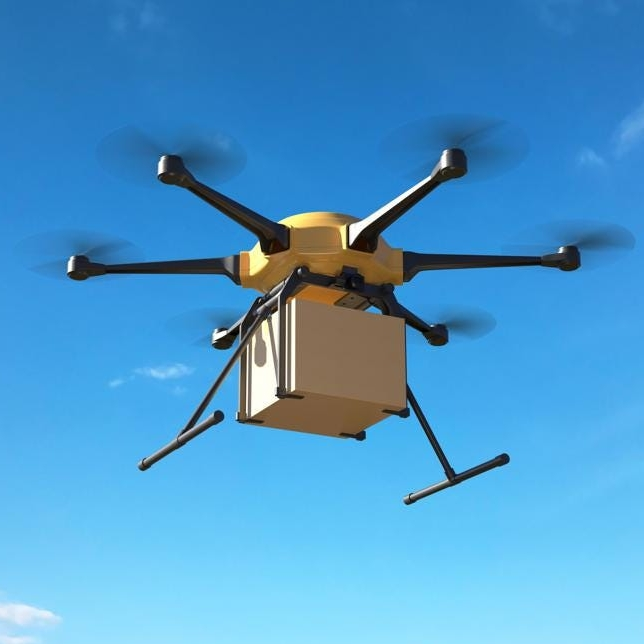
\includegraphics[width=0.9\linewidth]{rigid.jpg}
            \caption{Rigid connection \cite{Wolf2020}}
        \end{subfigure}
        \begin{subfigure}[t]{0.32\textwidth}
            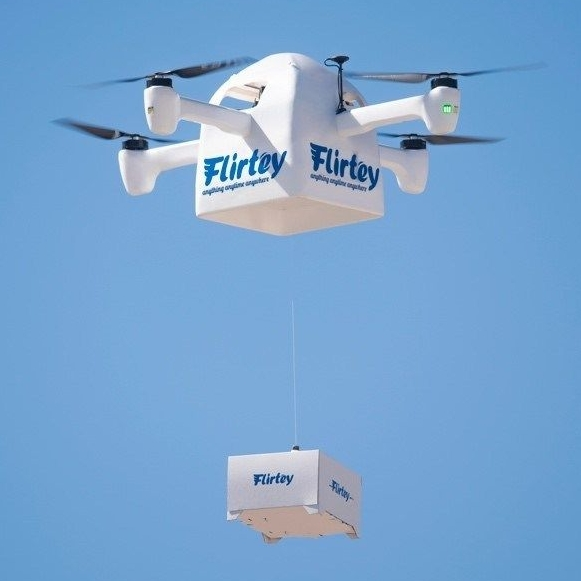
\includegraphics[width=0.9\linewidth]{suspended.jpg}
            \caption{Suspended cable \cite{Flirtey}}
        \end{subfigure}
        \begin{subfigure}[t]{0.32\textwidth}
            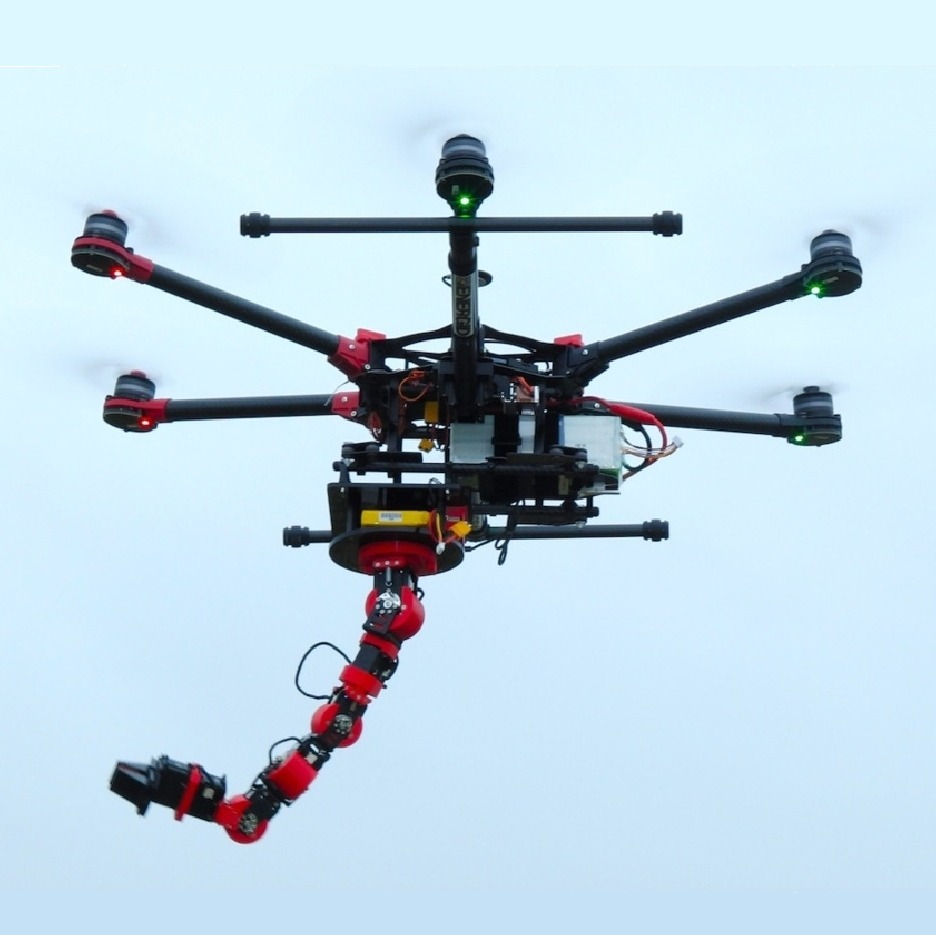
\includegraphics[width=0.9\linewidth]{actuated_payload_blue_bg.jpg}
            \caption{Robotic actuator \cite{Tardella2016}}
        \end{subfigure}
        \caption{Different multirotor payload configurations}
        \label{fig:rigid_suspended_actuated} 
    \end{figure}

    \subsection{Rigid connection payloads}

        \paragraph
        Payloads are often rigidly attached to a multirotor for transportation.
        This configuration is especially popular for commercial package deliveries \cite{San2018}.
        There is minimal relative movement between the multirotor and the rigidly connected payload, hence, the payload only affects the \gls{CoM}, the moment of inertia, and the aerodynamics of the vehicle.
        Often, the weight and size of the payload is unknown prior to flight.
        
        \paragraph
        Different control approaches have been proposed to deal with the altered flight dynamics for this applications, 
        including \gls{ARC} \cite{Min2011} and \gls{MRAC} \cite{Emran2015}.
        These control architectures mostly involve a parameter estimation algorithm to estimate the inertial parameters,
        and an adaptive control law based on the estimated parameters and predetermined dynamical model of the system.

        % \paragraph
        % \citet{Mellinger2011a} proposed an adaptive controller for a multirotor with a rigidly connected payload.
        % Least-squares estimation techniques were applied to estimate the inertial parameters of the payload.
        % A adaptive control law was then applied which uses the estimated parameters in the control law.
        % Experimental results showed acceptable trajectory tracking performance with the adaptive controller.

        \paragraph
        An advantage of rigidly connected payloads is that the flight dynamics is not altered significantly.
        The payload does not add a degree of freedom to the system and only the inertial parameters need to be accounted for.
        However, this configuration limits the shape and size of a potential payload, since
        the payload needs to be compatible with the vehicle gripper.
        The multirotor also needs to land or approach the payload very closely to attach to the load, which may be impractical in many applications.

    \subsection{Suspended payloads}

        \paragraph
        Figure~\ref{fig:real_suspended_payload_example} shows an example of a practical application of a suspended payload used during search and rescue missions.
        The shape and mass of the payload has an effect on the flight dynamics, but the payload is often unknown prior to flight.
        The control system should be able to account for these uncertainties and fly well despite the altered flight dynamics.

        \begin{figure}[htb]
            \centering
            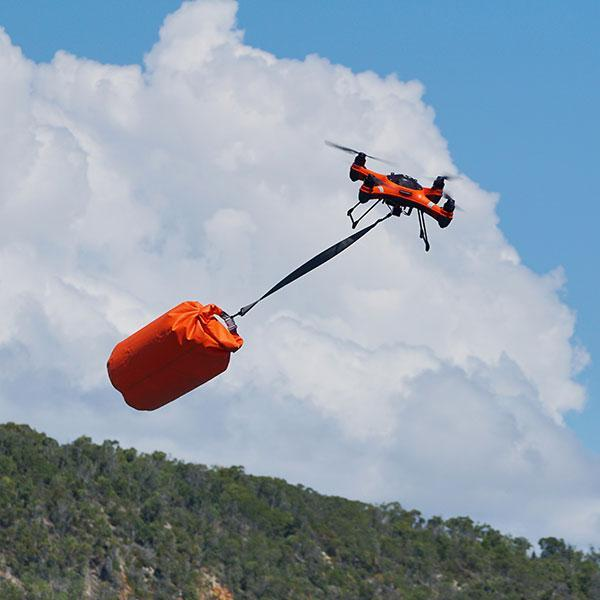
\includegraphics[width=0.45\linewidth]{real_suspended_payload_example.jpg}            
            \caption{A practical suspended payload used for search and rescue missions \cite{CompareCommander2020}}
            \label{fig:real_suspended_payload_example}
        \end{figure}

        \paragraph
        Various suspended payload configurations have been considered in literature.
        The classical suspended payload application involves a small payload suspended below the vehicle with rigid link \cite{Erasmus2020, Slabber2020, Guerrero-Sanchez2017, Klausen2017, Ichikawa2018, DeAngelis2019a}. 
        \citet{Kotaru2017} considered a suspended payload system with an elastic cable modelled as a spring-damper system.
        \citet{Tang2015a} modelled the multirotor-payload system with a hybrid dynamical model to consider aggressive manoeuvres where the cable transitions from taut to slack.
        The transportation of payload loads with flexible cables have also been studied, where the cable is modelled as a set of serially-connected rigid links  \cite{Goodarzi2015, Goodarzi2014, Kotaru2018}. 
        Furthermore, the control of a group of multirotors cooperatively transporting a suspended payload have also been considered in various studies \cite{Lee2015, Sanalitro2020, Klausen2014, Goodarzi2015}.
        
        \paragraph % This paragraph seems out of place and does not flow well
        From numerous examples in literature, it is clear that the control of multirotors with suspended payloads is a popular research topic.
        The cable-suspended payload configuration is very useful in situations where a multirotor cannot land, since the payload can be attached during hover.
        This configuration also has the advantage that a load can have an arbitrary shape or size as long as it has an attachment point for a cable.
        However, the suspended payload increases the degrees of underactuation of the system, which makes the control problem challenging \cite{Kotaru2018}.

        % ?? Fi author cite and [12-15] to rather [12,13,14,15]
\section{Control of multirotors with suspended payloads}

    \paragraph
    A major drawback of transporting a cable-suspended payload is that the payload is free to swing during flight, which effects the dynamics of a multirotor.
    Two main control strategies are applied in literature to stabilise a multirotor with a suspended payload, namely, trajectory generation and active vibration damping.
    Some methods combine the two methods into a single control architecture.
    Trajectory generation methods involve determining multirotor trajectories that result in minimal oscillations or specific payload trajectories.
    Active vibration damping controllers involve feedback controllers that apply a control law to actively counteract the swing of the payload.

    \subsection{Trajectory generation}

        \paragraph
        Trajectory generation methods for suspended payload systems are based on open-loop control techniques.
        The objective of these techniques is to determine a trajectory in which the multirotor motion would induces a specific payload trajectory to reduce oscillations or avoid obstacles.
        Numerous trajectory generation methods have been explored in literature for suspended payload transportation 
        \cite{Tang2015b, Geisert2016, Zeng2019, Xian2020, Starr2005, Palunko2012, Su2019, Palunko2013, Faust2013}. % ?? Maybe remove this long citation?

        \paragraph
        \citet{Zeng2019} and \citet{Tang2015b} applied differential flatness based trajectory planning methods for multirotors in obstacle-filled environments.
        Instead of only considering swing-reduction of the suspended payloads, these studies consider specific payload trajectories to avoid obstacles during aggressive motion.
        \citet{Xian2020} proposed an efficient online trajectory planning method without iterative optimizations.
        The swing-reduction performance of this method was also verified with experimental results.
        
        \paragraph
        Dynamic programming methods have also been implemented to generate swing-free trajectories with suspended payloads \cite{Starr2005, Palunko2012, Su2019}.
        These methods require accurate models of the plant dynamics and are sensitive to the accuracy of these models.
        \gls{RL} methods do not require prior models of the dynamics and have also been applied for swing-free trajectory generation \cite{Palunko2013, Faust2013}.
        \citet{Faust2013} implemented a \gls{RL} method for minimal swing trajectories which provides sufficient criteria to allow the learned policy to be transferred to a variety of different models, starting positions, and trajectories.
        Furthermore, this \gls{RL} trajectory generation method was verified with simulation and experimental results.
        % ?? Maybe continue this and explain more

        % Look for newer literature. ??

        % ?? Maybe add this
        % \paragraph 
        % A drawback of \gls{MPC} and \gls{RL} methods is that they rely on cost functions with tuning weights and linear constraints for obstacle avoidance.
        % \citet{Silveira2020} addressed this problem by implementing a \gls{RRT} algorithm that does not rely on cost functions and constraints for collision-free trajectories with a suspended payload.
        % However, this approach does not provide an optimal solution, but rather finds any collision-free trajectory as a solution. 

        \paragraph
        Input shaping is another open-loop control method applied for minimal swing control that is related to trajectory planning.
        This technique involves modifying a reference signal, usually with a set of timed impulses, to cancel oscillatory modes of the system \cite{Vaughan2008}.
        These techniques were originally designed for transporting suspended payloads using gantry systems \cite{Smith1957, Starr1983}.
        Later, these input shaping techniques were also applied for reduced swing control of 
        helicopters \cite{Bisgaard2008, Potter2011} and 
        multirotors \cite{Homolka2017, Sadr2014b, Fielding2019} that carry suspended payloads.

        \paragraph
        \citet{Ichikawa2018a} compared different input shaping techniques for velocity control of a quadrotor with a suspended payload in simulations.
        The specific input shaping techniques considered were: \gls{ZV}, \gls{NZV}, \gls{EI}, and 2-hump \gls{EI}.
        These methods convolve a baseline input command with precisely timed impulses based on the length of the suspended cable. 
        Simulation results showed that the input shapers significantly decreased the residual payload oscillations compared to a baseline velocity controller.
        It was highlighted that \gls{EI} and 2-hump \gls{EI} were more robust to cable length uncertainty than \gls{ZV} and \gls{NZV}.

        \paragraph
        \citet{Slabber2020} applied a notch filter to reduce cable-suspended payload oscillations for velocity control of a multirotor in simulation.
        \citet{Slabber2020} considered a system with unknown payload parameters.
        The unknown payload mass and cable length were estimated with \gls{RLS} and \gls{FFT} parameter estimators respectively and
        the natural frequency was calculated based on these estimates.
        The notch filter was applied to the velocity setpoint signal to suppress the frequency band containing this natural frequency. 
        \citet{Slabber2020} showed that a wider frequency band could be used to improve robustness against parameter uncertainty.
        It was shown in simulation that the notch filter attenuated the payload oscillations to a near swing free motion even with large parameter estimation errors \cite{Slabber2020}.
    
    \subsection{Active vibration damping controllers}

        % ?? Add pictures

        \paragraph
        Active vibration damping is a closed-loop control method where a feedback control law is applied that directly affects the payload states.
        These controllers are also referred to as swing damping controllers.
        Instead of finding a trajectory that reduces oscillations, these controllers follow a given trajectory as close as possible while trying to reduce payload oscillations.
        These controllers generally perform better than open-loop methods for systems with model uncertainties and external disturbances \cite{Liang2021}.
         
        % ?? Check if all citations refer to correct work. Sometimes copied wrongly

        % \paragraph
        % Different types of controllers have been proposed for active swing damping control of \glspl{UAV} with suspended payloads.
        % These controllers include \gls{LQR} \cite{Alothman2015}, geometric control \cite{Zeng2019a}, back-stepping control \cite{Mosco-Luciano2020, Allahverdy2021}, \gls{SMC} \cite{Martinez-Vasquez2020, Allahverdy2021}, \gls{H-inf} \cite{Rigatos2018}, \gls{RISE} \cite{Yang2018}, \gls{MPC} \cite{Son2017, Son2018, Son2019, Zurn2016, Alothman2018, Santos2016, Andrade2016, Alothman2018a, Trachte2014}.
        % Learning based control techniques like \gls{RL} \cite{Hua2021, Faust2014} and \gls{BFBEL} \cite{Muthusamy2021a} have also been implemented as closed-loop swing damping controllers.
        
        \paragraph
        Different types of controllers have been proposed for active swing damping control of \glspl{UAV} with suspended payloads.
        These controllers include: 
        \begin{itemize}[noitemsep]
            \item \gls{LQR} \cite{Alothman2015, Alothman2016, Alothman2018a, Alothman2018b, Trachte2014, Fan2015}, 
            \item Geometric control \cite{Zeng2019a}, 
            \item Back-stepping control \cite{Mosco-Luciano2020, Allahverdy2021}, 
            \item \gls{SMC} \cite{Martinez-Vasquez2020, Allahverdy2021}, 
            \item \gls{H-inf} \cite{Rigatos2018}, 
            \item \gls{MRAC} \cite{Erasmus2020}
            \item \gls{RISE} \cite{Yang2018}, 
            \item \gls{RL} \cite{Hua2021, Faust2014},
            \item \gls{BFBEL} \cite{Muthusamy2021a}, and
            \item \gls{MPC} \cite{Son2017, Son2018, Son2019, Zurn2016, Alothman2018, Santos2016, Andrade2016, Alothman2018a, Trachte2014}.
        \end{itemize}

        \paragraph
        \gls{LQR} is a popular optimal control technique and has often been used as a baseline controller to evaluate the performance of other swing damping controllers for multirotors with suspended payloads \cite{Trachte2014, Alothman2018a, Alothman2018b, Slabber2020, Alothman2016, Notter2016}.
        \citet{Erasmus2020article} proposed \gls{LQG} control for swing damping control of a multirotor with suspended cable.
        The payload state remained unmeasured and a \gls{EKF} was implemented for full-state estimation of the multirotor-payload system.
        The \gls{EKF} was combined with an \gls{LQR} full-state feedback controller to produce \gls{LQG} control.
        Simulation results showed good swing damping control with position step inputs despite the unmeasured payload state, external disturbances, sensor noise, and parameter uncertainty.

        \paragraph
        \citet{Slabber2020} implemented a \gls{LQR} controller augmented with a notch filter input shaper for improved swing damping performance.
        The notch filter was applied to the velocity step reference and the 
        \gls{LQR} was then applied with the filtered reference signal for swing-damping control.
        The \gls{LQR} was designed with integral action added to the velocity state to ensure zero steady-state velocity tracking. 
        Furthermore, this work involved estimating the unknown payload state with a vision-based estimator for use in the full-state feedback controller. 
        Simulation results showed that this controller provides good swing damping performance in the presence of external disturbances, sensor noise, and parameter uncertainty. 

        \paragraph
        \gls{MPC} is an optimal control technique related to \gls{LQR} that has also been applied to suspended payload systems.
        % \gls{MPC} solves control optimisation problem over a finite prediction horizon at every control interval based on a separately identifiable plant model \cite{Mayne2000}.
        \citet{Notter2016} implemented an \gls{MPC} for active swing damping control of a quadrotor with a suspended payload.
        A non-linear model of the quadrotor-payload system was linearised and discretised to apply a discrete, linear \gls{MPC} formulation.
        The physical parameters of the quadrotor, cable, and payload were assumed to be exactly known and the controller is tested with only one payload.
        The controller received a position trajectory reference and determined force setpoints to control the vehicle.
        Furthermore, constraints were applied to the heigh, attitude, and control inputs to ensure safe flight manoeuvres. 
        Simulation results showed superior trajectory tracking performance of the \gls{MPC} compared to a baseline \gls{LQR} controller.
        The \gls{MPC} simulation results were also verified with experimental results in an practical indoor environment.

        \paragraph
        \citet{Santos2018} implemented a robust tube-based \gls{MPC} for trajectory tracking and payload stabilisation of a tilt-rotor \gls{UAV} and suspended payload. 
        This approach consists of a pre-stabilising control policy for the nominal system and an additive control policy for the mismatch error. 
        The \gls{MPC} was applied for outer-loop position control, and a mixed $\mathcal{H}_2 / \mathcal{H}_\infty$ controller was applied for inner-loop attitude control.
        Simulation results showed ??
        It was also shown that this controller is robust against additive uncertainties from unmodelled dynamics, decoupling assumptions, linearization and discretisation simplifications.

        % \gls{MPC} can be viewed as
        % combination between open-loop and closed-loop strategies.
        % Replanning.
        % Open-loop vs closed-loop: 
        % https://www.sciencedirect.com/science/article/pii/S0005109817302327
        % https://engineering.stackexchange.com/questions/18992/open-loop-versus-closed-loop-model-predictive-control

    
    % ?? Lit study: include different types of \gls{MPC}, e.g. DMC, MAC
    % ?? different types of models \cite{}, 
    % ?? See \cite{Garcia1989} for good example of different implementations with different models

    % ?? Table of literature
    % Unknown payloads
    % what is unknown

    % See data driven is scarce?
    % therefore data driven.
    % MPC is a good method of applying model

\section{Multirotor control with unknown dynamics}

    \paragraph
    Unknown states.
    Erasmus.
    Get more cites from erasmus.
    Mention adaptive.
    Mention robust.


    \subsection{Unknown parameters}
        
        \paragraph

    
    \subsection{Unknown models}

        \paragraph
        Learning-based methods have also been proposed for multirotors with suspended payloads.
        \citet{Hua2021} develops a non-linear control strategy embedded with \gls{RL} for position control and simultaneous swing suppression.
        Experimental results showed that this method provided reliable swing suppression control in situations with model uncertainties, parameters drift, and external disturbances.
        
        \paragraph

        \paragraph
        RL

        \paragraph
        MPC with system identification

        \paragraph
        DMD

\section{Summary} 
        
    \paragraph
    Where does my work fit in.

    The major contribution of this work

% \section{System Design}
% Blok diagram
% komponente

}


